\documentclass[titlepage=firstcover, captions=tableheading]{scrartcl}
\usepackage{microtype}
\usepackage{amsmath}
\usepackage{polyglossia}
\usepackage{graphicx}
\usepackage{booktabs}
\usepackage{siunitx}
\usepackage{hyperref}
\usepackage{caption}
\usepackage{float}
\setdefaultlanguage{german}
\title{V703 Das Geiger-Müller-Zählrohr}
\author{
Connor Magnus Böckmann \\ email: \href{mailto:connormagnus.boeckmann@tu-dortmund.de}{connormagnus.boeckmann@tu-dortmund.de}
\and Tim Theissel \\ email: \href{mailto:tim.theissel@tu-dortmund.de}{tim.theissel@tu-dortmund.de}}
\begin{document}
\maketitle
\newpage
\tableofcontents
\newpage
\section{Zielsetzung}
In diesem Versuch wird das Geiger-Mueller-Zaehlrohr untersucht, welches ionisierende Strahlung detektieren und messen kann. Es ist in der Lage einen elektrischen Impuls auszugeben, sollte ein \alpha- oder \beta-Teilchen im Inneren detektiert werden. Dieser Impuls kann dann von einem Impulszaehler gezaehlt werden und die pro Zeit- und Flaecheneinheit einfallenden Teilchen bzw. Quanten messen und dadurch die Intensitaet bestimmen. 
\section{Theoretische Grundlagen}
\subsection{Aufbau und prinzipielle Funktionsweise}
Der prinzipielle Aufbau des Zaehlrohrs ist in \ref{Fig:Aufbau} zu sehen.
\begin{figure}[H]
    \centering
    \includegraphics{"Aufbau_Geiger.png"}
    \caption{Aufbau eines Geiger-Mueller-Zaehlrohrs mit Endfenster\\ Aus: Anleitung V703 Seite 220}
    \label{Fig:Aufbau}
\end{figure}
 \noindent Das Zaehlrohr besteht aus einem Stahlzylinder mit dem Radius $r_k$, welcher die Kathode darstellt. In seinem Inneren befindet sich ein Draht, welcher die Anode (Radius $r_a$) darstellt. Der Zylinder ist versiegelt und mit einem Gasgemisch gefuellt. Durch das Anlegen einer ausseren Spannung U (ca. 300 bis 2000V) bildet sich ein elektrisches, radialsymmetrisches Feld aus. Die Feldstaerke betraegt im Abstand r von der Mittelachse $E(r)=\frac{U}{r\ln(\frac{r_k}{r_a})}$.
 Wenn ein geladenes Teilchen in das Zaehlrohr eintritt, wird es in dem E-Feld beschleunigt. Diese Beschleunigung steigt bei Annaeherung an den Draht mit $\frac{1}{r} \text{mit} (r_a < r < r_k)$. Theoretisch kann diese als beliebig gross werden, wenn nur der Drahtradius $r_a$ hinreichend klein gewaehlt wird.\\
 Sollte nun ein geladenes Teilchen ins Zaehlrohr gelangen, bewegt es sich so lange durch den Gasraum bis seine Energie durch Ionisation aufgebraucht ist. Da eine Ionenpaarbildung im Mittel nur etwa 26eV benoetigt, gegenueber einer Teilchenenergie von etwa 100keV, ist die Anzahl der positiven Ionen und Elektronen proportional zur Energie des ins Zaehlrohr eingefallenen Teilchens. Die angelegte Spannung hat nun einen grossen Einfluss auf die nach der Primaerionisation stattfindenden Prozesse. Eine Visualisierung findet sich in dem Diagramm in \ref{Fig:Spannung}.
 \begin{figure}[H]
    \centering
    \includegraphics[width=0.6\textwidth]{"Spannung_Geiger.png"}
    \caption{Anzahl der erzeugten Ionenpaare gegenueber der angelegten Spannung\\ Aus: Anleitung V703 Seite 221}
    \label{Fig:Spannung}
\end{figure}
\noindent Das Diagramm laesst sich dabei in verschiedene Bereiche einteilen. Zu Beobachten ist zum Beispiel der Bereich fuer sehr kleine Spannungen. Dabei werden die Ionen nicht stark genug beschleunigt, um den Draht zu erreichen. Viele rekombinieren sich vorher bereits (Bereich I). Je groesser die Spannung wird, desto groesser wird die Wahrscheinlichkeit, dass die Ionen sich nicht vor Erreichen des Drahtes rekombinieren. Es erreichen somit quasi alle Elektronen den Draht. In diesem Bereich ist der Ionisationsstrom zwischen Kathodenzylinder und Anodendraht proportional zur Energie und Intensitaet der einfallenden Teilchen. Dieser Zustand nennt sich Ionisationskammer und ist in Bereich II zu sehen. Zur tadellosen Funktion wird hierbei aber eine grosse Strahlungsintensitaet benoetigt. Bei noch hoerer Spannung wird die Feldstaerke in Drahtnaehe so gross, dass die entstehenden Elektronen zwischen zwei Zusammenstoessen genuegend Energie aufnehmen, um ihrerseits andere Gasteilchen ionisieren zu koennen. Dieser Vorgang nennt sich Stossionisation. Unter ausreichend grosser Spannung koennen die freigesetzten Elektronen selbst andere Teilchen ionisieren. Es bildet sich eine so genannte Townsend-Lawine. Hier ist nun auch die pro Teilchen einfallende Ladung gross genug, um sie als Ladungsimpuls zu messen. Durch die vorhandene Proportionalitaet zwischen der Ladung Q und der Teilchenenergie, laesst sich am Ladungsimpuls ein Mass fuer die Teilchenenergie festmachen. Eine Apparatur, die sich diese Proportionalitaet zu Nutze macht, nennt sich Proportionalitaetszaehlrohr (Bereich III).
Bei wiederum hoeheren Spannungen U ist die Ladung nicht mehr proportional zur Primaerionisation. Dieser Bereich nennt sich Ausloesebereich (Bereich IV). In diesem Bereich arbeitet ein Geiger-Mueller-Zaehlrohr unter normalen Bedingungen. Statt einer lokalen Elektronenlawine breitet sich die Lawine nicht nur in radialer Richtung, sondern auch entlang des Drahtes aus. Ausgeloest wird dieser Prozess durch die in der primaeren Lawine entstandenen UV-Photonen, welche durch die Anregung von Argon-Atomen im Fuellgas freisetzen. Diese Photonen koennen sich auf Grund ihrer Ladungsneutralitaet auch senkrecht zum E-Feld bewegen. Ihre Energie, welche sie durch Zusammenstoesse abgeben koennen, bildet den Grundstein fuer neue Elektronenlawinen im vollstaendigen Zaehlvolumen. Die am Draht gemessene Ladung haengt dann nicht mehr von der ersten Ionisation ab, sondern bloss vom Volumen des benutzten Zaehlrohrs und der angelegten Spannung. Bei dieser Spannung kann das Zaehlrohr nur noch als Intensitaetsmessgeraet benutzt werden. Eine Energiemessung ist nicht mehr moeglich. Dafuer kann die freigesetzte Ladung eines einfallenden Teilchens nun auf Grund ihrer nun relativ grossen Groesse mit geringem elektronischem Aufwand gut gemessen werden. Der so genannte Ausloesebereich beginnt in \ref{Fig:Spannung} dort, wo \alpha- und \beta-Kurve in einander uebergehen. Dort ist der Ladungsimpuls abgekoppelt vom Ionisationsvermoegen der einfallenden Strahlung.
\subsection{Totzeit und Nachentladungen}
Die entstehenden positiven Ionen haben eine bedeutend hoehere Masse als die Elektronen, weshalb sie deutlich langsamer abwandern. Sie halten sich also laenger im Raum zwischen Anode und Kathode. Aus diesem Grund bilden sie eine temporaere, radialsymmetrische, positive Raumladung aus. Diese wird auf Grund der zylindrischen Form des Rohrs auch Ionenschlauch genannt. Dadurch wird kurzzeitig fuer eine Zeit T die Feldstaerke in Drahtnaehe soweit herab, dass praktisch keine Stossionisation mehr moeglich ist. In dieser Zeit ist das Zaehlrohr nicht in der Lage eintreffende Teilchen zu detektieren, weshalb man diese Zeit auch Totzeit T nennt. Der Zustand loest sich durch Wandern der positiven Ladung in Richtung des Mantels auf. Die normale Feldstaerke stellt sich wieder her nachdem die Ionen vollstaendig neutralisiert wurden. Diese Zeit der Wiederherrstellung des Normalzustandes nennt sich treffenderweise Erholungszeit $T_E$, welche sich an die Totzeit anschliesst, bis das Zaehlrohr wieder unter Normalbedingungen detektieren kann.\\
Auf der Manteloberflaeche koennen die auftreffenden Ionen, durch ihre Neutralisationsenergie, Elektronen freisetzen. Diese Sekundaerelektronen werden zum Messdraht hin beschleunigt durch das E-Feld und sorgen auf diesem dann fuer ein erneutes Ausloesen des Messgeraets. Dadurch kann durch ein einzelnes eintreffendes Teilchen mehrere Entladungen am  Zaehlrohrdraht hervorgerufen werden. Diese zusaetzlichen Entladungen nennen sich Nachentladungen. Der zeitliche Abstand der Nachentladungen entspricht der Laufzeit $T_L$ der Elektronen von der Zylinderwand zum Draht. Diese Nachentladungen sind sehr unerwuenscht, da sie das Vorhandensein von ionisierender Strahlung vortaeuschen. Sie sollten also so weit wie moeglich unterbunden werden, was durch eine kleine Beimengung von Alkoholdaempfen zum Fuellgas gut gelingt, denn diese Alkoholdämpfe werden von den Edelgasionen ionisiert und wandern dann zur Kathode. Das Gute daran ist, dass die Alkoholionen an der Kathode keine Elektronen emittieren. Es gibt also keine weiteren Entladungen und die Messung wird nicht durch weitere Elektronen, die von der Kathode aus kommen beeinflusst.
\subsection{Charakteristik des Zaehlrohrs}
Die Charakteristik eines Geiger-Mueller-Zaehlrohr wird gegeben durch eine Auftragung der eintreffenden Teilchenzahl N gegen die Betriebsspannung U. In etwa sieht eine Charakteristik so aus:
\begin{figure}[H]
    \centering
    \includegraphics[width=0.6\textwidth]{"Charakteristik_Geiger.png"}
    \caption{Charakteristik eines Geiger-Mueller-Zaehlrohres bei konstanter Strahlungsintensitaet \\ Aus: Anleitung V703 Seite 224}
    \label{Fig:Charakteristik}
\end{figure}
\noindent Der Ausloesebereich beginnt hierbei etwa bei der Spannung $U_E$. Der linear steigende, abgeflachte Teil nennt sich Plateau. Die Steigung in diesem Bereich der Kurve ist bestenfalls moeglichst klein. Idealerweise waere diese also null, was aber nicht erreichbar ist. Diese Unmoeglichkeit ruegt von vereinzelten Nachentladungen her, welche trotz des Alkoholdampfes vorkommen. Am Ende des Plateaus nimmt die Zahl der Nachentladungen extrem zu, was den starken Anstieg erklaert. Je hoeher die Qualitaet des Zaehlrohres, desto laenger und flacher ist das Plateau.\\
Nach Ende des Plateaus geht das Zaehlrohr in den BEreich der selbststaendigen Gasentladung ueber. Dort zuendet ein einzelnes ionisierendes Teilchen eine Dauerentladung. Dies ist sehr schaedlich fuer das Zaehlrohr auf Grund der hohen Stromdichten und wird das Messgeraet schnell zerstoeren, sollte also auf jeden Fall vermieden werden.
\subsection{Ansprechvermoegen eines Zaehlrohres}
Das Ansprechvermoegen eines Zaehlrohres ist ein Mass dafuer wie wahrscheinlich es ist, dass ein einfallendes Teilchen auch tatsächlich detektiert wird. Fuer \alpha- und \beta-Teilchen ist das Ansprechvermoegen nahezu 100\%. Allerdings muss dazu natuerlich gewaehrleistet sein, dass die Teilchen auch tatsaechlich ins Innere des Zaehlrohres gelangen. Da diese Teilchen sehr wahrscheinlich mit Materie wechselwirken, werden sie im Metallmantel des Zaehlrohres absorbiert. Aus diesem Grund gibt es Endfensterzaehlrohre, welche am Ende des Volumens von einer duennen Mylar-Folie verschlossen werden. Diese kann selbst von \alpha-Teilchen durchdrungen werden. Ein solches Endfensterzaehlrohr ist in \ref{Fig:Aufbau} dargestellt.\\
Bei Photonen hingegen liegt das Ansprechvermoegen bei geringen Werten von etwa 1\%. Das folgt aus der geringen Wechselwirkungswahrscheinlichkeit von Photonen mit hoher Energie mit Materie. Die Nutzung eines Geiger-Mueller-Zaehlrohres zur Detektion von \gamma-Strahlung ist also nur bei hohen Intensitaeten dieser moeglich und sinnvoll. 
\section{Experimementelle Untersuchungen am Zaehlrohr}
Fuer die gemachten Messungen wurde die im folgende skizzierte Messapparatur verwendet.
\begin{figure}[H]
    \centering
    \includegraphics[width=0.6\textwidth]{"Apparatur_Geiger.png"}
    \caption{Aufbau der Messapparatur \\ Aus: Anleitung V703 Seite 226}
    \label{Fig:Apparatur}
\end{figure}
\noindent Ueber den Widerstand R fliesst die am Zaehldraht gesammelte Ladung Q ab. Ein Spannungsimpuls wird erzeugt. Nach Auskoppelung im Kondensator C wird dieser verstaerkt und im Zaehlgeraet gezaehlt. Auf dem Schirm eines Oszillographen kann dieser Impuls dann sichtbar gemacht werden.
\subsection{Aufnahme der Charakteristik}
Ein \beta-Strahler wird vor das Einlassfenster des Messgeraets gestellt. Dabei wird die Zaehlrate gemessen und in Abhaengigkeit von der Betriebsspannung gesetzt. Zu Beachten ist dabei, dass die Zaehlrate 100 pro Sekunde nicht ueberschreitet. Hierbei sollte den Moeglichkeiten entsprechend sehr genau gemessen werden, da die Plateausteigeung sowieso schon sehr gering ist. Desweiteren darf beim verwendeten Zaehlrohr die Betriebsspannung nicht ueber 700 Volt hinausgehen. Andernfalls geraet das Zaehlrohr in den Bereich der bereits genannten selbststaendigen Gasentladung. Bei Missachtung folgt schnell die Zerstoerung des Messgeraetes. 
\subsection{Sichtbarmachung von Nachentladungen}
Es sollen die Nachentladungen mit einem Oszilloskop qualitativ sichtbar gemacht werden. Dazu wird die Intensitaet der Strahlenquelle soweit gesenkt, dass auf dem Bildschirm des Oszilloskop waehrend der Laufzeit des Strahls von links nach recht kein weiterer Impuls zu sehen ist. Die Zaehlrohrspannung muss so gering sein, dass die Wahrscheinlichkeit fuer NAchentladungen sehr gering ist. Hier werden 350V verwendet. Nun wird die Zaehlrohrspannung schrittweise bis au 700V erhoeht. Der zeitliche Abstand zwischen der Primaer- und Nachentladung wird gemessen.
\subsection{Bestimmung der Totzeit mit der Zwei-Quellen-Methode}
Die Totzeit T sorgt fuer eine registrierte Impulsrate $N_r$, welche immer kleiner ist als die tatsaechliche Anzahl der eingedrungenen Teilchen $N_W$. Wenn $N_r$ Impulse pro Zeiteinheit registriert werden, so ist das Geraet fuer den Bruchteil $TN_r$ nicht in der Lage Teilchen zu regestrieren, weshalb es nur im Bereich $1-TN_r$ messbereit ist. Die wahre Impulsrate ist also:
\begin{equation}\label{2}
    N_W=\frac{Impulsrate}{Messzeit}=\frac{N_rt}{(1-TN_r)t}=\frac{N_r}{1-TN_r}
\end{equation}
Nun kann mit dieser Formel die Totzeit bestimmt werden. Dazu werden zwei Radioaktive Praeparate benoetigt. Es wird dazu zuerst die Zaehlrate $N_1$ des Messgeraets mit dem ersten Praeparat gemessen. Danach wird ein zweites Praeparat hinzugenommen ohne die Postion des ersten Praeparates zu veraendern. Die Zaehlrate $N_{1+2}$ wird gemessen. Daraufhin wird das erste Praeparat entfernt und die Messrate $N_2$ gemessen.\\
Ohne Totzeit waere 
\begin{equation}
    N_{1+2}=N_1+N_2\nonumber
\end{equation}
Stattdessen laesst sich aber beobachten, dass $N_{1+2}<N_1+N_2$ ist. Gemaess \ref{2} gilt fuer die von den Praeparaten emittierten und ins Zaehlrohr eingedrungenen Teilchen
\begin{align}
    N_{W_1}&=\frac{N_1}{1-TN_1}\nonumber\\
    N_{W_2}&=\frac{N_2}{1-TN_2}\nonumber\\
    N_{W_{1+2}}&=\frac{N_{1+2}}{1-TN_{1+2}}\nonumber
\end{align}
Ausserdem ist $N_{W_{1+2}}=N_{W_1}+N_{W_2}$. Daraus ergibt sich dann
\begin{equation}\label{Totzeit}
    \frac{N_{1+2}}{1-TN_{1+2}}=\frac{N_1}{1-TN_1}+\frac{N_{1+2}}{1-TN_{1+2}}
\end{equation}
Da die Groessen $N_1$, $N_2$ und $N_{1+2}$ bekannt sind kann aus \ref{Totzeit} die Totzeit T bestimmt werden. T laesst sich naeherungsweise schreiben als 
\begin{align}
    T\approx\frac{N_1+N_2-N_{1+2}}{2N_1N_2}
\end{align}
\subsection{Messung der freigesetzten Ladungsmenge pro Teilchen}
Wie in \ref{Fig:Apparatur} kann mit einem empfindlichen Strommessgeraet der mittlere Strom des Zaehlrohrs gemessen werden. 
\begin{align}
    \bar{I}:=\frac{1}{\tau}\int_0^\tau \frac{U(t)}{R} \text{dt}\nonumber\\
    \text{(\tau>>T)}\nonumber
\end{align}
Daraus laesst sich nun die pro eindringendes Teilchen freigesetzte Ladungsmenge bei bekannter Impulszahl pro Zeiteinheit berechnen. Es gilt der Zusammenhang 
\begin{align}
    \bar{I}=\frac{\Delta Q}{\Delta t}Z\nonumber
\end{align}
Dabei ist \Delta Q die pro Zeitintervall \Delta t transportierte Ladungsmenge, wenn Z die Anzahl der registrierten Teilchen ist.

\documentclass[titlepage=firstcover, captions=tableheading]{scrartcl}
\usepackage{microtype}
\usepackage{amsmath}
\usepackage{polyglossia}
\usepackage{graphicx}
\usepackage{booktabs}
\usepackage{siunitx}
\usepackage{hyperref}
\usepackage{caption}
\usepackage{float}
\setdefaultlanguage{german}

\begin{document}
    
\section{Auswertung}

\subsection{Geometrische Abmessungen}

In der Folgenden Tabelle werden die geometrischen Abmessungen der verwendeten Kupferproben dargestellt.
Dabei gibt es für die Kupferfolie eine Höhe (H), eine Breite(b) und eine Dicke (d) sowie einen Durchmesser (D) und eine Länge (L) des Kupferdrahtes.

\begin{center}
    \captionof{table}{Geometrische Abmessungen in cm}
    \begin{tabular}{lllll}
        \toprule
        H & b & d & D & L \\
        \midrule 
        0.026 & 0.028 & 0.00043 & 0.000263 & 173 \\
        \bottomrule
    \end{tabular}
\end{center}

\subsection{Widerstand}

Der Widerstand wurde bei der Durchführung des Versuchs direkt mit einem Multimeter gemessen.
Dafür musste lediglich das Messgerät an den Kupferdraht angeschlossen werden und mit den richtigen Einstellungen zeigt es einen Widerstand von 9.7 \Omega \; an.

\subsection{Hall Effekt}

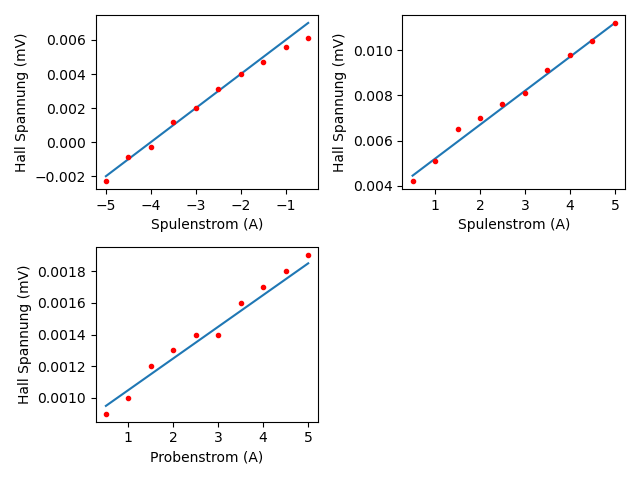
\includegraphics{plothall.png}

In den Koordinatensystemen sind die gemessenen Hall-Spannungen aufgetragen.
Zu den Geaphen ist zu sagen, dass auf der x-Achse entweder der Spulenstrom oder der Probenstrom abgebildet wird.
Die jewils andere Stromstärke wird konstant bei 5A gehalten.

\subsection{Ladungsträger pro Volumen n}

n lässt sich mit der Formel ? brechnen.
Um mit dieser Formel zu rechnen ist es notwendig, die Magnetfeldstärke in abhängigkeit der Stromstärke zu kennen.
Dieser Zusammenhang ist durch die Messwerte gegeben.
Ebenso sind die gemessenen Hall-Spannungen für diese Rechnung notwendig.

Daraus lässt sich die Ladungsdichte bestimmen.

\begin{minipage}{\linewidth}
    \centering
\captionof{table}{Ladungsdichte der Kupferprobe}
\begin{tabular}{ll}
    \toprule
    Stromstärke (A) & Magnetfeldstärke (T) \\
    \midrule
    0.5 &  
    1   &     
    1.5 &  
    2   &  
    2.5 &  
    3   &  
    3.5 &  
    4   &  
    4.5 &  
    5   &      \\
    \bottomrule
    
\end{tabular}
\end{minipage}

\end{document}
%\end{document}
